\newpage
\section{Precision Placement Test}
\label{sec:Precision Placement Test}

The \iaterm{Precision Placement Test}{PPT} requires high precision while detecting, grasping, transporting and placing objects. Three objects are initially placed on a 10cm service area and must be placed into the respective cavity on a precision placement table as described in Section~\ref{sec:Precision Placement}. The position of the cavities on the table is random, meaning robots must recognize the correct cavity for an object class. Objects must completely pass the table surface to count as placed successfully.

Reduced placement points will be awarded if an object gets stuck in the correct cavity hole or lying on the correct cavity tile. It is allowed to perform recovery strategies if a robot can detect objects that have not fallen through (e.g. force fitting, swiping, unstuck), but only if the respective object is already on the correct tile.
It is not allowed to move or damage the cavities during this process. See section \ref{ssec:PlacingObjects} for more detailed placing information.

As navigation is not the focus of this test, the source location will be close to the precise placement table and no obstacles are placed inside the arena. The robot does not have to move to the FINISH location. The run ends once the third object has been successfully placed or a rule violation has been called by the referees.

%The same arena as for the Basic Manipulation Test is used. In case that the arena does not already include a modified service area as shown in Figure \ref{fig:ppt_plattform}, it will be added only for this particular test.
%\paragraph{Purpose and Focus of the Test}
%The purpose of the \iaterm{Precision Placement Test}{PPT} is to assess the robot's ability to grasp and place objects into object-specific cavities. This demands advanced perception abilities (to recognize the correct cavity for each object) and manipulation abilities (to grasp and place the object in such a manner that it fits into the cavity).
%
%\paragraph{Manipulation Objects}
%The manipulation objects used in this test are defined by the instances described in Table~\ref{tab:Instances}.
%
%\paragraph{Task}
%The objective of the task is to pick the objects which are placed on one service area and make a precise placement in the corresponding cavity at the service area with the special PPT platform (an example configuration is illustrated in Figure \ref{fig:ppt_plattform}). 
%
%\begin{figure}
%\centering
%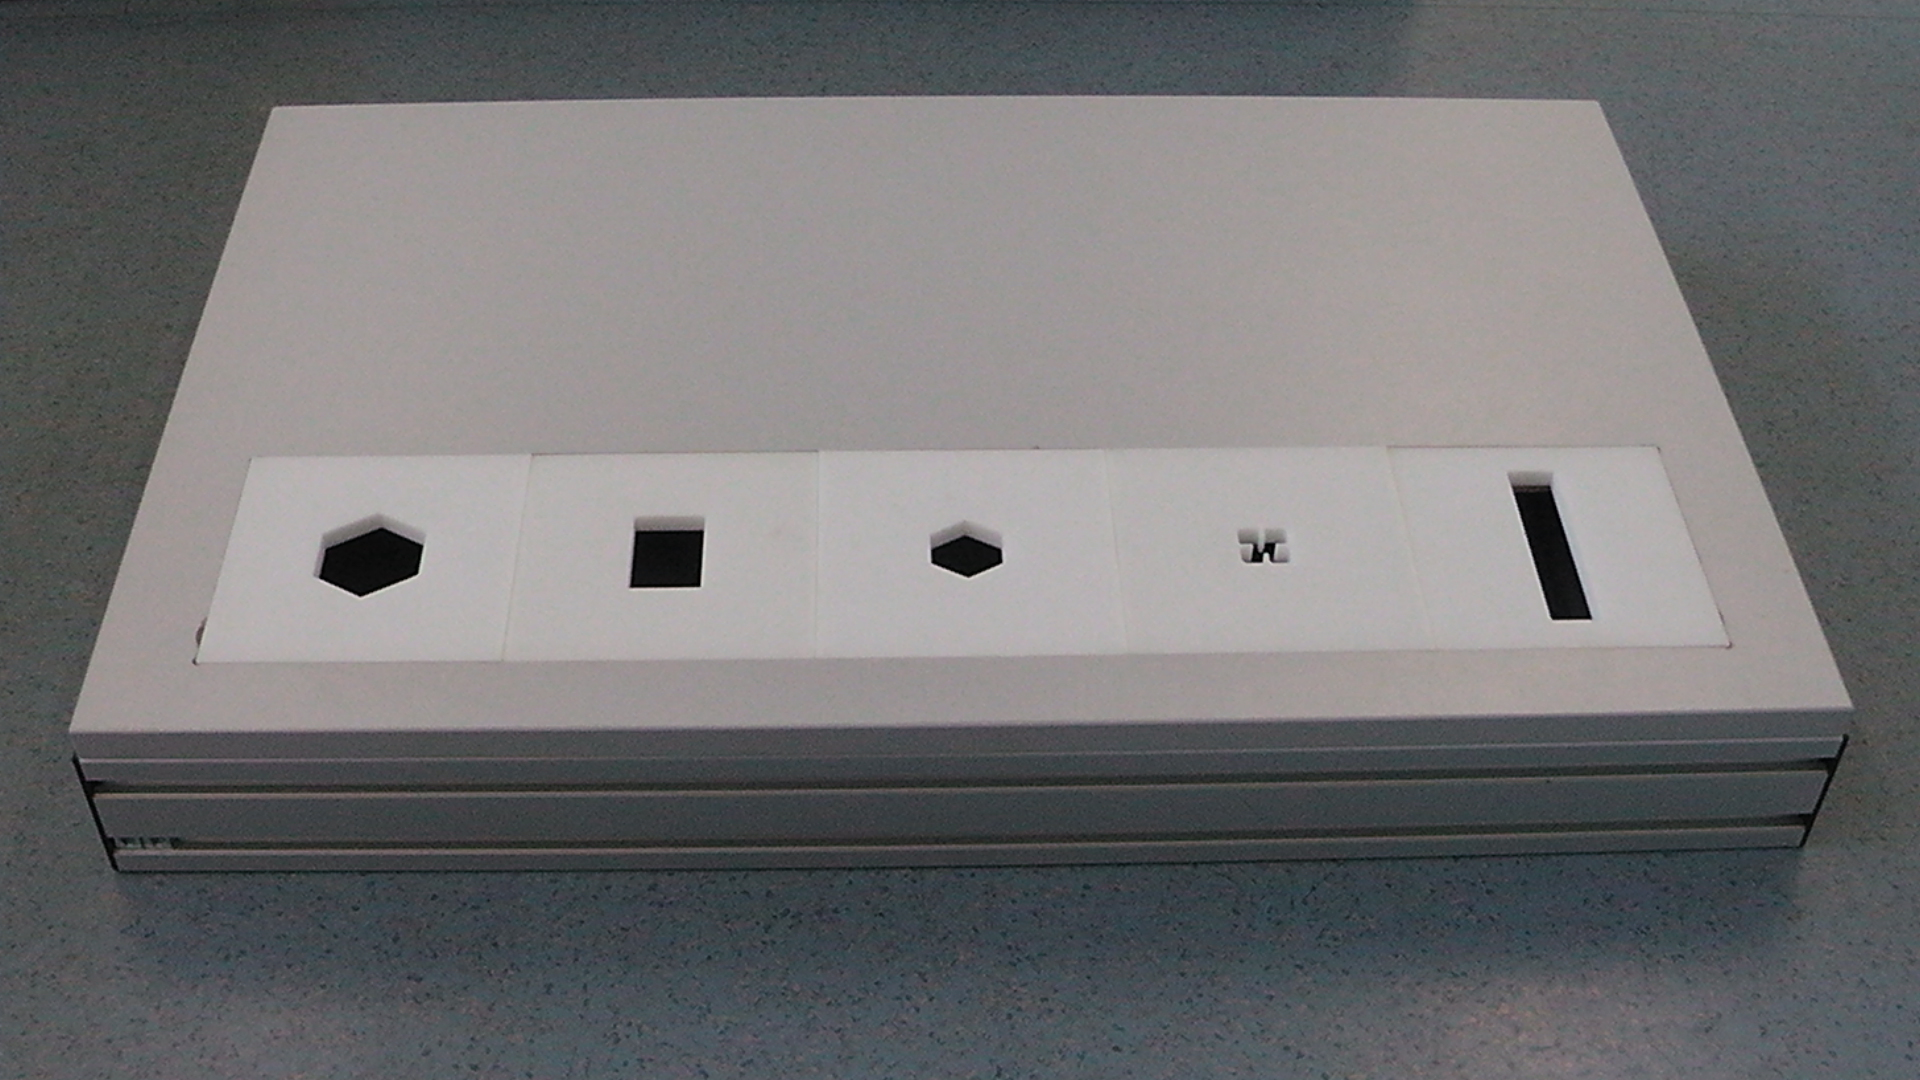
\includegraphics[width=0.6\textwidth ]{./images/ppt_plattform.jpg}
%\caption{The PPT platform including five cavity tiles}
%\label{fig:ppt_plattform}
%\end{figure}
%
%The task consists of multiple grasp and place operations, possibly with base movement in between, which will, however, be short. Note that the placement of the object in the cavity is finished when the object is fallen into the cavity (i.e. at least some part of the object has to touch ground floor underneath the cavity).
%
%%
%%\subsection{Complexity Levels}
%%
%%All Complexity Options from BMT apply.
%%
%%\subsubsection{PPT Orientation Complexity (bonus factor = 0.2):}
%%The cavities can be placed in all orientations.
%%\subsubsection{PPT Rotation Complexity (bonus factor = 0.2):}
%%The cavities can be placed in all orientations.
%
%\paragraph{Rules}
%The following rules have to be obeyed:
%
%
%%\subsection{Scoring}
%%Points are awarded as follows:
%%
%%\begin{itemize}
%%\item 50 points are awarded for successfully grasping an object.
%%\item 100 points are awarded for successfully placing a manipulation object into the correct cavity.
%%\item 50 points are awarded if the task specification has been completely fulfilled. The task is considered as fulfilled if all objects have been dropped in the right cavity. The robot does not have to leave the arena.
%%\item a penalty of -50 points is given for each object which has been dropped into the wrong cavity
%%\item The reached points of a test will be multiplied with a defined complexity factor depending on the previously chosen complexity level.
%%\end{itemize}
%
%
